\documentclass{beamer}
\usepackage[latin1]{inputenc}
%\usetheme[noshadow,nonav,nologo]{NYU}
\usetheme[numbers]{NYU}
\usepackage{amsmath}
\usepackage{amsfonts}
\usepackage{amssymb}
\usepackage{color, colortbl}
\usepackage{graphicx}
\usepackage{subfigure}
\usepackage{caption}
\usepackage{subcaption}
\usepackage{epstopdf}

\makeatletter
\newcommand{\thickhline}{%
    \noalign {\ifnum 0=`}\fi \hrule height 2pt
    \futurelet \reserved@a \@xhline}

\title{Learning Representations from Temporal Data}
\date{October 29, 2014} 
\author{Ross Goroshin}

\begin{document}
\begin{frame}
\titlepage
\end{frame}


\begin{frame}
\frametitle{Objectives of Research}  
\begin{itemize}
\item Characterize \emph{generically} useful properties of features  
\item Design loss functionals which explicitly or implicitly promote desirable feature characteristics 
\item Self contained evaluation criteria, requiring no external oracle
\end{itemize}
\end{frame}

\begin{frame}
\frametitle{Supervised Deep Feature Learning} 
\centerline{\includegraphics[scale=0.1]{./images/clarifai.png}} 
\centerline{\includegraphics[scale=0.2]{./images/modeep.jpg}}
\centerline{Works in practice, scales in depth, stable, immediate results} 
\end{frame}

\begin{frame}
\frametitle{Data in High Dimensions} 
\centerline{\includegraphics[scale=0.2]{./images/DQE/structure.png}}
\centerline{\includegraphics[scale=0.35]{./images/DQE/spaces.png}}
Dependencies among variables imply a low dimensional structure
\end{frame} 

\begin{frame}
\small
\frametitle{Models of Data} 
\begin{center} 
\begin{tabular}{c||c|c|c|c}
Algorithm & Model & Encode & Decode & Learning\\
\thickhline
\cellcolor{red}PCA & Linear &\checkmark & \checkmark & $W_D = W_E ^T$\\
\hline
\cellcolor{red}ICA & Linear &\checkmark & \checkmark & $W_D = W_E ^T$\\
\thickhline
\cellcolor{yellow}Sparse Coding & Locally Linear &\checkmark(\$) & \checkmark & inference, $W_D$ \\
\hline
\cellcolor{yellow}CBP & Osculating Sphere &\checkmark(\$) & \checkmark & inference, $W_D$ \\
\hline 
\cellcolor{yellow}PSD \& LISTA & Locally Linear &\checkmark & \checkmark & hybrid, $W_D$\\
\hline
\cellcolor{orange}Metric Learning & Nonlinear & \checkmark & X & $W_E$ only\\
\hline
\cellcolor{green}Auto-Encoders & Nonlinear & \checkmark & \checkmark & $W_E$ \& $W_D$ 
\end{tabular} 
\end{center} 

\begin{center}
\begin{tabular}{c|c|}
\hline
\cellcolor{red} \hspace{10 mm} & De-correlation/Independence  \\
\cellcolor{yellow} \hspace{10 mm} & Sparsity \\
\hline
\cellcolor{orange} \hspace{10 mm} & Metric Learning/Restricted Metric Learning  \\
\hline
\cellcolor{green} \hspace{10 mm} & All of the Above \\
\hline
\end{tabular}
\end{center} 
\end{frame} 

\begin{frame}
\frametitle{Preserving Information} 
\centerline{\includegraphics[scale=0.3]{./images/DQE/autoenc.png}}
Optimizing desirable properties ('contrastive terms') of the representation alone often leads to degenerate solutions. 
\begin{itemize}
\item Directly reconstruct the input from it's latent representation (PCA, Auto-encoders, Sparse Coding) 
\item Assign high probability to your data, low probability everywhere else (Max-Likelihood Models) 
\item Enforce the features to have unit variance (kurtosis-based ICA, slow-feature analysis) 
\item Push the representation of samples apart (DrLIM, nuclear norm)   
\end{itemize} 
\end{frame} 

\begin{frame}
\frametitle{Auto-Encoders/Dictionary Learning} 
\begin{center} 
\begin{itemize} 
\item Auto-Encoders replace the 'inference' step of dictionary learning with a learned feed forward function 
\item In addition to reconstruction additional terms are included to induce desirable properties in the representation
\item Example: \textbf{Sparse Coding / Sparse Auto-Encoder} 
\end{itemize} 
$\min_{z, W} \frac{1}{2} \|x - W z \|_2 ^2 + \lambda \| z \|_1$\\
\begin{flushleft} Dictionary Learning is to alternate between:  \end{flushleft} 
\begin{eqnarray} 
z_{k+1} &=& shrink(z_k - \eta_1 \nabla_{z_k}\frac{1}{2} \|x - W_k z_k \|_2 ^2)\\
W_{k+1} &=& W_k - \eta_2 \nabla_{W_k}\frac{1}{2} \|x - W_k z_k \|_2 ^2
\end{eqnarray}
\begin{flushleft} Auto-Encoder formulation usually uses SGD to solve: \end{flushleft} 
$\min_{W_e, W_d} \frac{1}{2} \|x - W_d F_{W_e}(x) \|_2 ^2 + \lambda \| F_{W_e} \|_1$
\end{center} 
\end{frame} 

\begin{frame} 
\begin{center}
\frametitle{Sparsity and Independence} 
\includegraphics[scale = 0.3]{./images/DQE/L1.png}
\includegraphics[scale = 0.3]{./images/DQE/ICA.png}\\
Left: Minimize $L_1$, goal: sparsity\\ Right: Maximize kurotsis, goal: independence\\
(If individual code elements have low enetropy (sparsity), code variables should be as independent as possible in order to maximize information capacity)
\end{center}
\end{frame}

\begin{frame}
\frametitle{Parameterizing $F_{W_e}$: LISTA Inference}  
\begin{center} 
\includegraphics[scale = 0.3]{./images/LISTA/LISTA.png} \\
$S = I - \frac{1}{L} W_d ^T W_d$ and $W_e = \frac{1}{L} W_d ^T$
\end{center} 
\begin{itemize}
\item{Learned ISTA is a method for approximating the inference step by a feed forward network} 
\item{Originally designed/tested to perform inference in a \emph{fixed} dictionary. Does it also work when jointly learning the dictionary, i.e. as an encoder?} 
\end{itemize} 
\end{frame} 

\begin{frame}
\frametitle{LISTA Inference} 
\centerline{\includegraphics[scale=0.35]{./images/LISTA/code_pred.png}}
\end{frame} 

\begin{frame}
\frametitle{LISTA Inference} 
\centerline{\includegraphics[scale=0.35]{./images/LISTA/LISTA_loss_min.png}}
\begin{itemize}
\item LISTA works best when minimizing the loss (not code prediction error) directly with a \emph{fixed} dictionary 
\item It it is not beneficial when learning the dictionary  
\end{itemize} 
\end{frame} 

\begin{frame}
\frametitle{Contractive/Saturating Regularization} 
Contractive regularization
\begin{itemize}
\item Penalize the norm of the Jacobian of the representation, w.r.t. the inputs at each sample
\item This promotes stability (invariance) at the samples in all directions except in the tangent space of the manifold 
\item Let $f(\cdot)$ be a point-wise nonlinear activation function
\item{$L_{CAE} = \sum_{x \in D_n} \|x-W_d f(W_e x)\|_2 ^2 + \lambda \sum_{ij} \left(\frac{\partial f_j(W_e x)}{\partial x_i} \right)^2$ }
\end{itemize} 
Saturating regularization
\begin{itemize}
\item Assuming $f(\cdot)$ has zero gradient regions, introduce a complimentary function $f_c(\cdot)$ to $f(\cdot)$ 
\item $f_c(\cdot)$ is the distance transform to the nearest gradient region 
\item The motivation is to obtain an implicit parameterization of the data manifold. The data manifold is implicitly embedded in the reconstruction error function
\item{$L_{SAT} = \sum_{x \in D_n} \|x-W_d f(W_e x)\|_2 ^2 + \lambda f_c(W_e x)$ }
\end{itemize} 
\end{frame} 

\begin{frame}
\frametitle{Saturating Auto-Encoders} 
\centerline{\includegraphics[scale=0.35]{./images/SATAE/compliments.png}}
\centerline{\includegraphics[scale=0.3]{./images/SATAE/toy_shrink.png}}
\end{frame} 

\begin{frame}
\frametitle{Saturating Auto-Encoders} 
\centerline{\includegraphics[scale=0.35]{./images/SATAE/viz_nonlin.png}}
\begin{itemize} 
\item Shrink and ReLU saturating auto-encoders are equivalent to $L_1$ regularized auto-encoders with corresponding nonlinearities 
\item Saturating auto-encoders with sigmoid-like activation functions regularize the representation by promoting binary codes 
\end{itemize} 
\end{frame} 

\begin{frame}
\frametitle{Saturated Linear Activations} 
\centerline{\includegraphics[scale=0.3]{./images/SATAE/toy_sat_linear_reg.png}}
\end{frame} 

\begin{frame} 
\frametitle{Shrink/ReLU Activations} 
\begin{center} 
\includegraphics[width=0.15\textwidth]{./images/SATAE/CIFAR_shrink01.png} \hspace{1cm} 
\includegraphics[width=0.18\textwidth]{./images/SATAE/strokes_full.png}
\end{center} 
\end{frame} 

\begin{frame}
\frametitle{Saturated Linear Activations} 
\begin{center} 
\includegraphics[width=0.15\textwidth]{./images/SATAE/CIFAR_sat_linear03.png} \hspace{1cm} 
\includegraphics[width=0.18\textwidth]{./images/SATAE/MNIST_sat_linear_full.png}
\end{center} 
\end{frame} 

\begin{frame}
\frametitle{Lessons} 
\begin{itemize} 
\item Contractive regularization is effective only within a small ball around each sample (same with denoising auto-encoder)
\item Saturated-linear auto-encoder does not work for certain datasets (e.g. MNIST)
\item Parameterization is important. Which portions of the input space are assigned a higher energy? Do we have any reasonable hope of seeing any samples from the test set there?  
\end{itemize} 
\end{frame}

\begin{frame}
\frametitle{The Role of Time} 
\centerline{\includegraphics[width=0.55\textwidth]{./images/TAE/vision.png}} 
Time is a one dimensional parametrization of the data-manifold, neighbors in time should be neighbors in feature space.
\end{frame} 

\begin{frame}
\frametitle{Learning a Temporally Coherent Metric} 
\begin{center}
\includegraphics[scale=0.5]{./images/TAE/toyplane.png} 
\includegraphics[scale=0.5]{./images/TAE/toyplane2.png} 
\includegraphics[scale=0.5]{./images/TAE/toyplane3.png} \\
\includegraphics[scale=0.5,trim = 120 100 130 70, clip]{./images/TAE/drlim1.pdf}
\includegraphics[scale=0.5,trim = 120 100 130 70, clip]{./images/TAE/drlim2.pdf}\\
\includegraphics[scale=0.5,trim = 120 100 130 70, clip]{./images/TAE/drlim3.pdf} 
\includegraphics[scale=0.5,trim = 120 100 130 70, clip]{./images/TAE/drlim4.pdf}
\begin{equation} 
\nonumber
L(x_t,x_{t'},W)=\left\{
                \begin{array}{ll}
                 \|G_W(x_t) - G_W(x_{t'})\|_p, &\text{if}~|t-t'| = 1  \\
                 \max(0,m-\|G_W(x_t) - G_W(x_{t'})\|_p) &\text{if}~|t-t'| > 1
                \end{array}
              \right.
\end{equation} 
\end{center} 
\end{frame} 


\begin{frame}
\frametitle{Learning Sparse and Slow Features} 
\begin{equation}
\nonumber 
L(x_t,x_{t'},W)= \sum_{\tau = \{t,t'\}} \left(\|W_d h_\tau - x_\tau\| + \alpha|h_t| \right)+\beta \sum_{i=1}^K \left| \|h_t\|^{P_i} - \|h_{t'}\|^{P_i} \right|
\end{equation} 
Where the vector of hidden activations for the sample at time $t$ is denoted by $h_t=f(W_ex_t)$, and $\|h_t\|^{P_i}$ denotes a local $L_2$ pooling over the neighborhood $P_i$ 
\end{frame}

\begin{frame}
\frametitle{Learning Sparse and Slow Features} 
\begin{center} 
\includegraphics[scale=0.33]{./images/TAE/slow_dec_pooling_sub.png} \hspace{0.5cm} 
\includegraphics[scale=0.33]{./images/TAE/slow_dec_l1_pooling.png}
\end{center} 
\centerline{Learned bases with (right) and without (left) $L_1$ penalty} 
\end{frame}

\begin{frame}
\frametitle{Spatially Coherent Features} 
\centerline{\includegraphics[scale=0.6,trim = 20 350 300 50, clip]{./images/TAE/diagram.pdf}} 
\begin{itemize}
\item What criterion should determine the values of $\alpha$ and $\beta$? 
\item What is the correct trade-off between discriminability and invariance? 
\end{itemize} 
\end{frame}

\begin{frame}
\frametitle{Datasets} 
\centerline{\includegraphics[scale=0.4]{./images/TAE/youtube.png}} \vspace{0.1cm}
\centerline{Train frames = 125,000, Test frames = 23,337 (1,626 unique scenes)} 
\centerline{\includegraphics[scale=0.4]{./images/TAE/cifar.png}} 
\centerline{Train images = 50,000, Test images 10,000}
\end{frame}

\begin{frame}
\frametitle{Scene Precision-Recall} 
\centerline{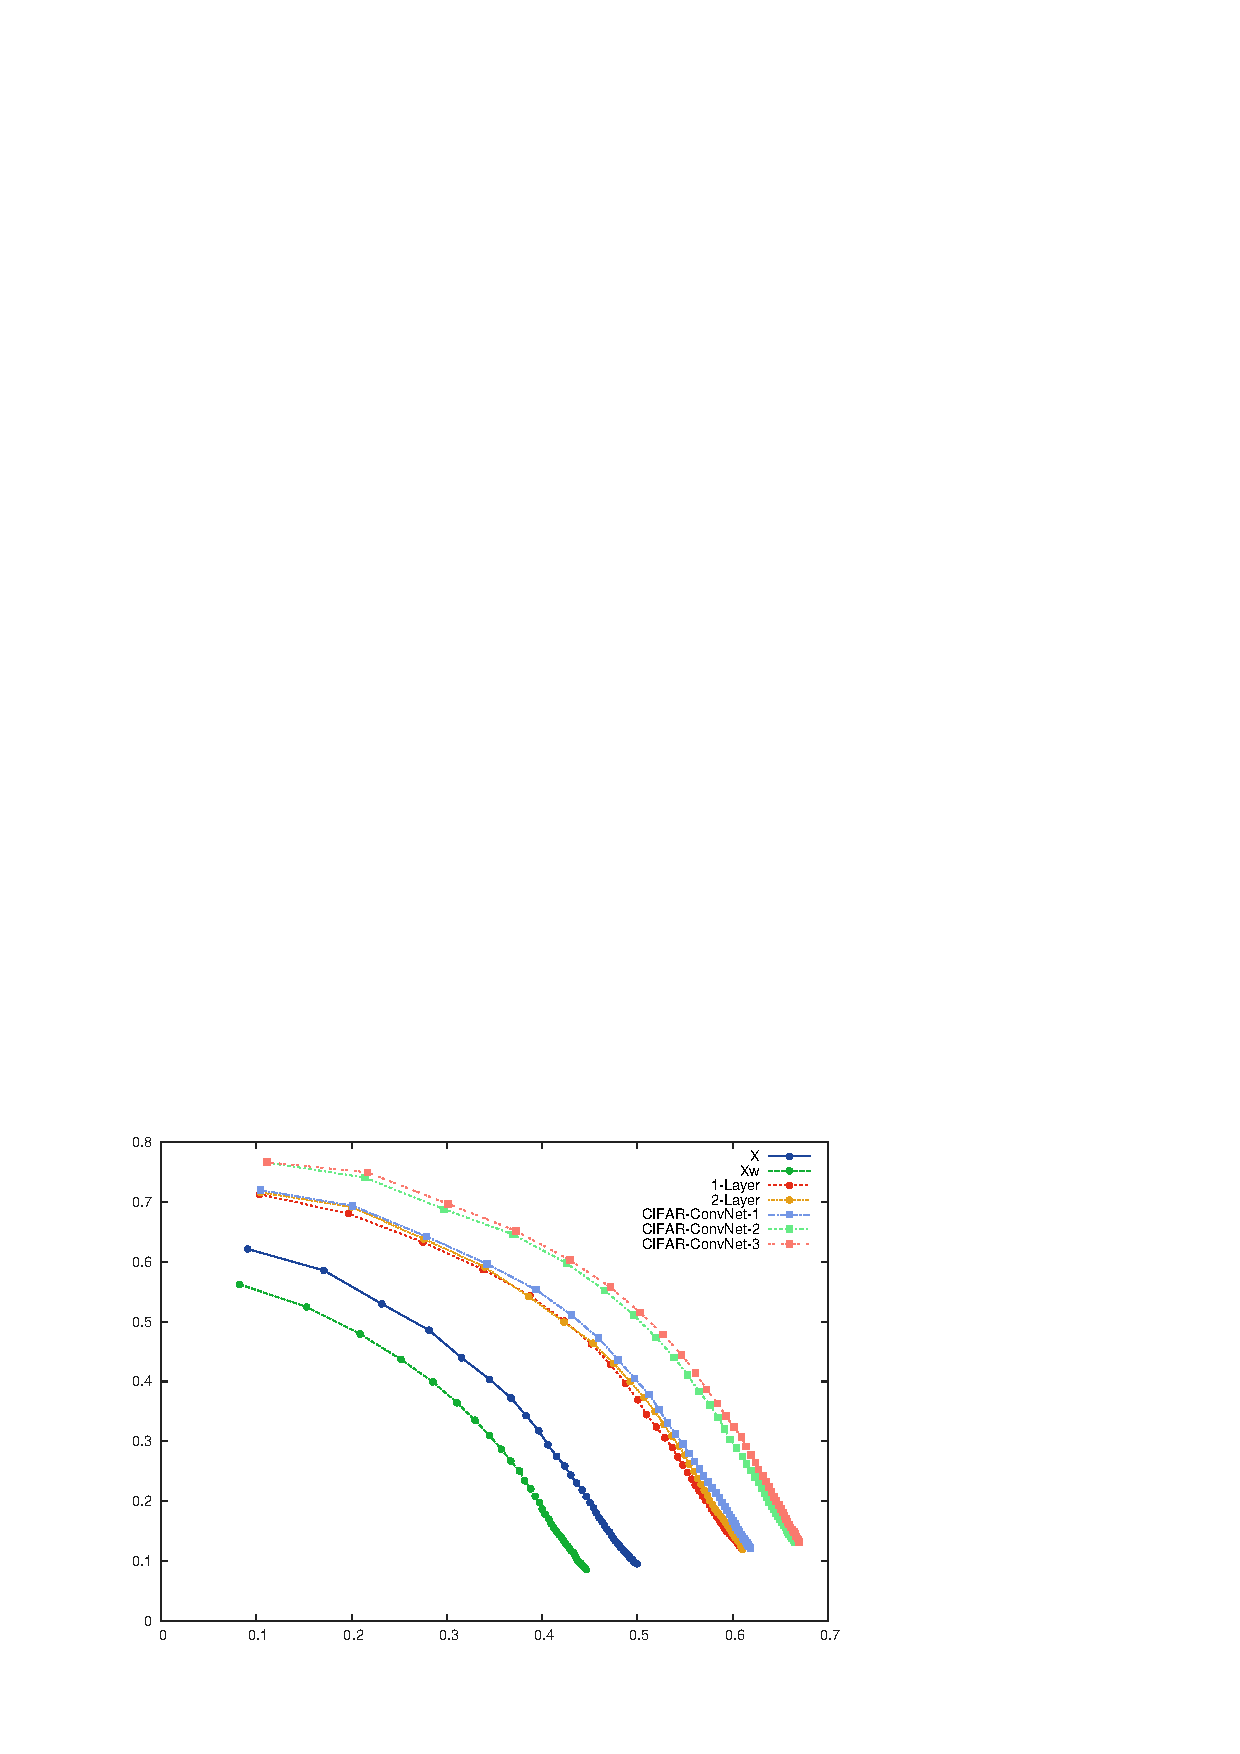
\includegraphics[scale=0.8]{./images/TAE/AUC_time.pdf}} 
\end{frame}

\begin{frame}
\frametitle{Scene Precision-Recall} 
\centerline{\includegraphics[scale=0.6]{./images/TAE/AUC_slowness.pdf}} 
\end{frame}

\begin{frame}
\frametitle{Class Precision-Recall} 
\centerline{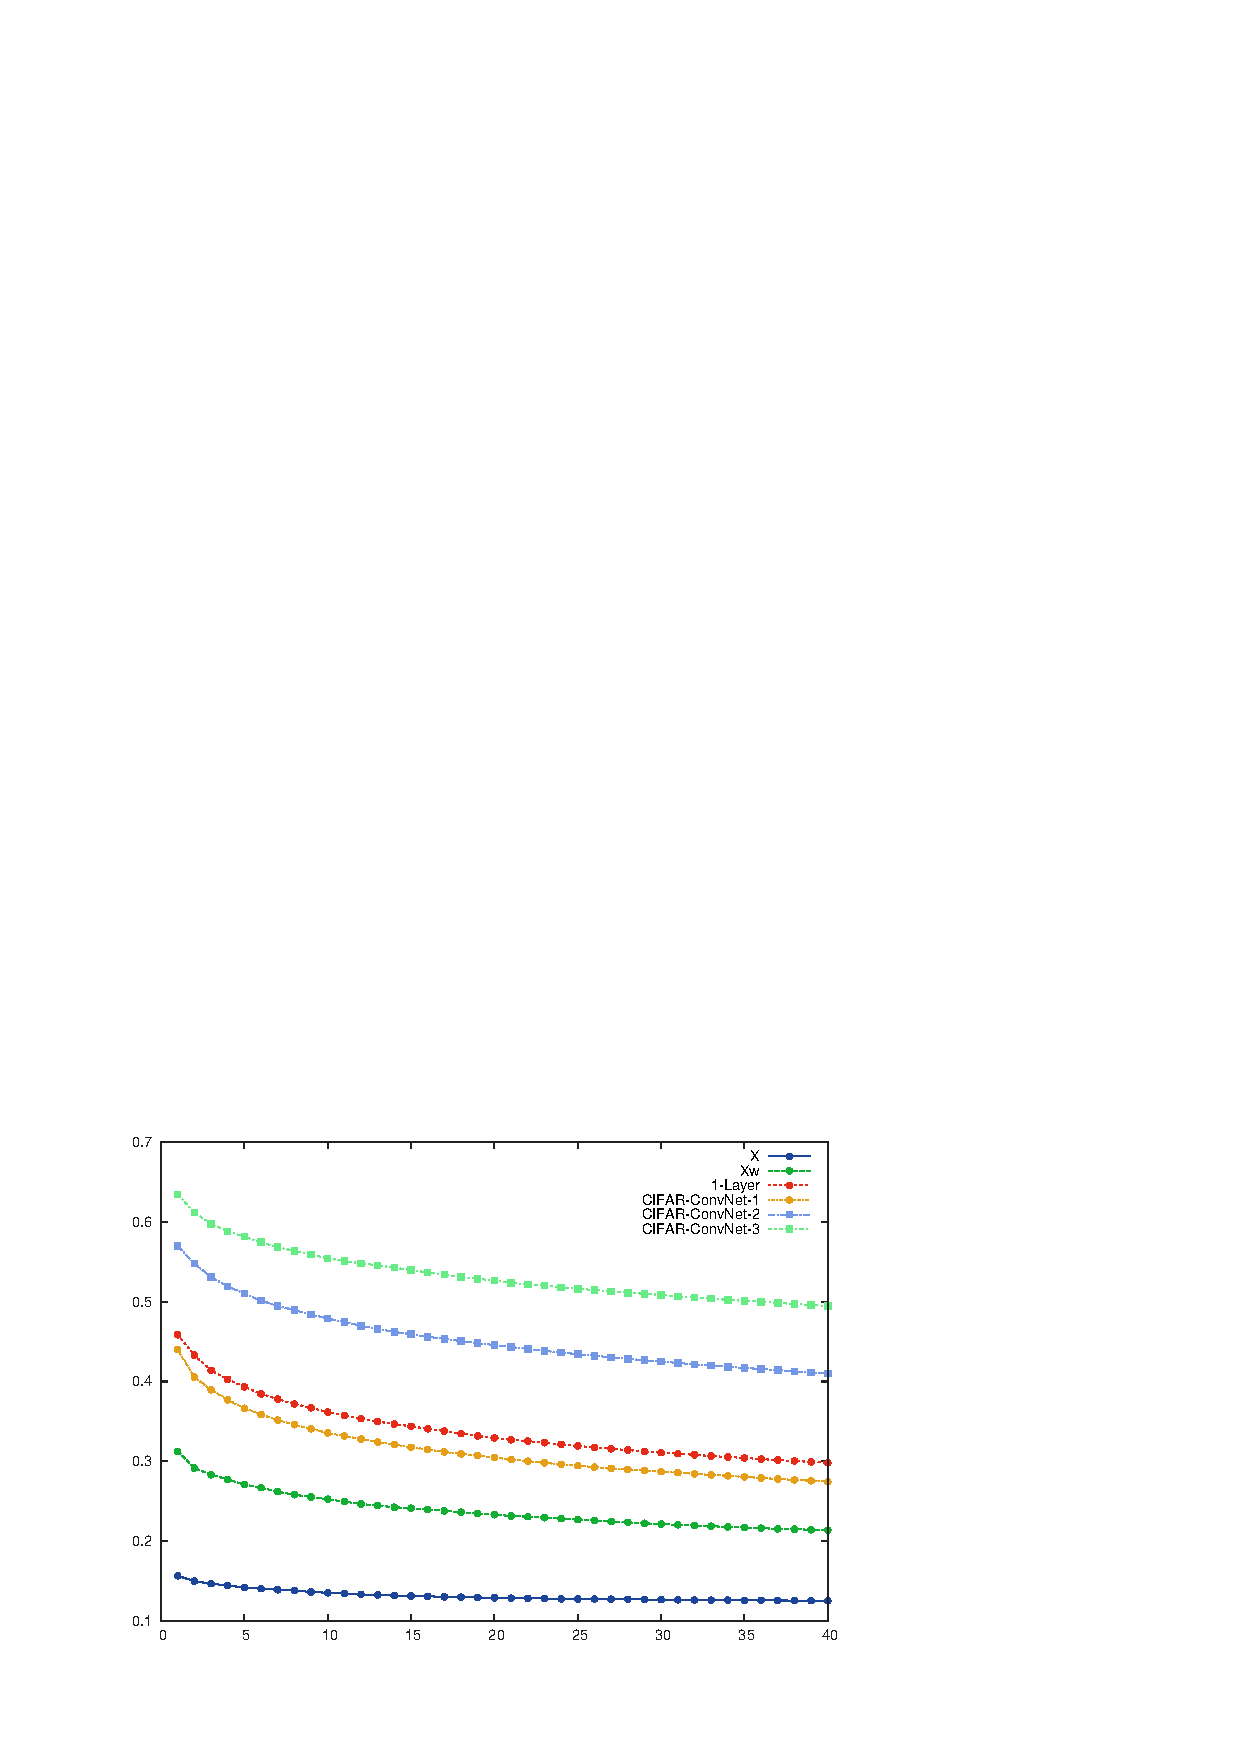
\includegraphics[scale=0.8]{./images/TAE/AUC_class.pdf}} 
\end{frame}

\begin{frame}
\frametitle{Learned Filter Banks} 
\begin{center} 
\includegraphics[scale=1.0]{./images/TAE/dec_small_slow.png} \hspace{0.5cm} 
\includegraphics[scale=1.0]{./images/TAE/dec_large_slow.png} \\
\includegraphics[scale=0.3]{./images/TAE/act_small_slow.png} \hspace{0.5cm} 
\includegraphics[scale=0.3]{./images/TAE/act_large_slow.png} 
\end{center} 
\end{frame}

\begin{frame}
\frametitle{Relationship between Performance on Two Datasets} 
\centerline{\includegraphics[scale=0.55]{./images/TAE/AUC_32.png}}
\end{frame}

\begin{frame}
\frametitle{Relationship between Performance on Two Datasets} 
\centerline{\includegraphics[scale=0.55]{./images/TAE/AUC_48.png}}
\end{frame}

\begin{frame}
\frametitle{Relationship between Performance on Two Datasets} 
\centerline{\includegraphics[scale=0.55]{./images/TAE/AUC_64.png}}
\end{frame}

\begin{frame}
\frametitle{Relationship between Performance on Two Datasets} 
\centerline{\includegraphics[scale=0.55]{./images/TAE/AUC_all.png}}
\end{frame}

\begin{frame}
\frametitle{Shortcomings of the Model} 
\begin{itemize} 
\item Does not regularize/output where (phase), only the what (magnitude) 
\item Indirect control on the informativeness of the representation because reconstruction is enforced \emph{before} pooling 
\item Equivalent to reconstructing from a pooling operator which outputs all the moments
\item Phase is unregularized    
\item Difficult to train multiple layers greedily  
\end{itemize} 
\end{frame}

\begin{frame}
\frametitle{Other Temporal Objectives} 
Learn a representation that is information preserving and locally linearizes temporal trajectories 
\centerline{\includegraphics[scale=0.3]{./images/NewStuff/manifolds.pdf}}
Let $\phi(x_t)$ be the feature-space representation of the sample at $t$ \\
\centerline{$\|2\phi(x_t)-\phi(x_{t-1})-\phi(x_{t+1})\|$}
\end{frame} 

\begin{frame}
\frametitle{Pooling with Phase} 
Magnitude: $m_i = \max\limits_{z_j \in N_i(z_j)} z_j$ \hspace{0.25cm} or \hspace{0.25cm} $m_i = \frac{1}{\beta} log\left( \sum\limits_{z_j \in N_i} e^ {\beta z_j} \right)$ \\
Phase: $p_k = \frac{e^{\beta z_k}}{\sum\limits_{z_j \in N_i} e^{\beta z_j}}$ \\
First moment of the phase: $\mu_i = \sum \limits_{p_j \in N_i} x_j p_j$ \\
\begin{itemize}
\item Assign a topology on the support $N_i$, and let $x_j$ be a monotonic function of $j$
\item $\mu_i$ correspond to the offset within $N_i$
\item Constant speed translations of the activations along their support correspond to \emph{linear variations} in $\mu$
\item Pooling across feature maps parameterizes arbitrary transformations
\end{itemize} 
\end{frame} 

\begin{frame} 
\frametitle{Applications}
\underline{Supervised}  
\begin{itemize} 
\item With spatial pooling $\| \mu_i - \mu_j \|$ is the distance between the activations of features $i$ and $j$  
\item End-to-end training of parts models
\end{itemize} 
\underline{Unsupervised}  
\begin{itemize} 
\item Minimize $\|2\mu_t-\mu_{t-1}-\mu_{t+1}\|$, provided that $m_{t-1}>0$, $m_t>0$, and $m_{t+1}>0$, and minimize $|m_{t}-m_{t-1}|$
\item This induces the pool group activations to be piecewise constant, while linearizing the phase within each group
\item Phase moments and magnitude can be used to generate a reconstruction of the input
\end{itemize} 
\end{frame} 

\begin{frame} 
\frametitle{Supervised-Like Training with Time}
Is it possible to conceive of an objective that implicitly forces temporal linearization? 
\centerline{\includegraphics[scale=0.4]{./images/NewStuff/frame_order.pdf}}
\end{frame} 

\begin{frame}
\centerline{
\huge
\emph{Thank you}} 
\centerline{
\emph{(Questions?)}}
\vspace{10 mm} 
\end{frame}

\end{document}


